
\documentclass[english]{cccconf}
% The preceding line is only needed to identify funding in the first footnote. If that is unneeded, please comment it out.
\usepackage{cite}
\usepackage{amsmath,amssymb,amsfonts}
\usepackage{algorithmic}
\usepackage{graphicx}
\usepackage{textcomp}
\usepackage{xcolor}
%\documentclass[usemulticol,english]{cccconf}
\usepackage[comma,numbers,square,sort&compress]{natbib}
\usepackage{epstopdf}
\usepackage{booktabs}
\usepackage{multirow}
\usepackage{amsmath,amssymb,amsfonts}
\usepackage{stfloats}
\usepackage{bm}
\usepackage[ruled,linesnumbered]{algorithm2e}

\begin{document}
	
	\title{Title}
	
	\author{San Zhang\aref{sjtu}, Si Li\aref{sjtu}, Wu Wang\aref{sjtu}^*}
	
	% Note: the first argument in the \affiliation command is optional.
	% It defines a label for the affiliation which can be used in the \aref
	% command. If there is only one affiliation for all authors, then the
	% optional argument in the \affiliation command should be suppressed,
	% and the \aref command should also be removed after each author in
	% \author command, in this case the affiliation will not be numbered.
	
	
	\affiliation[sjtu]{Department of Automation, Shanghai Jiao Tong University, Shanghai 200240, China}
	\affiliation{*E-mail: wangwu@sjtu.edu.cn}  
	
	
	\maketitle


\begin{abstract}
This document is a model and instructions for \LaTeX.
This and the IEEEtran.cls file define the components of your paper [title, text, heads, etc.]. *CRITICAL: Do Not Use Symbols, Special Characters, Footnotes, 
or Math in Paper Title or Abstract.
\end{abstract}

\keywords{component, formatting, style, styling, insert}



Introduction
Therefore, choosing a suitable carrier spacing is the key to achieving high precision 5G+TSN synchronization.The problem can be reduced to a trade-off problem between synchronization accuracy and bandwidth utilization, where the bandwidth utilization can be expressed as follows:
\begin{equation}
	\eta=\frac{12\cdot N_{RB}\cdot \triangle F}{B}
\end{equation}
where $N_{RB}$ is the number of RBs and $B$ is the bandwidth of the network.So we can construct an optimization problem to find the optimal carrier spacing:
\begin{equation}
	\begin{split}
		&\min_{\triangle F} \,\, \omega_1 \cdot T_c+\omega_2 \cdot \frac{1}{\eta} \\
		&s.t.\quad  \left\{\begin{array}{lc}
			T_{cmin}\leq T_c \leq T_{cmax}\\
			B_{min}\leq B \leq B_{max}\\
			N_{RB}\leq 273\\
		\end{array}\right.
	\end{split}
\end{equation}
where $\omega_1$ and $\omega_2$ are the weights of synchronization accuracy and bandwidth utilization, respectively, and users assign their sizes according to their needs. By this method, the synchronization error can be minimized without causing a large impact on the original communication quality of the 5G network.


Industrial communication networks require high availability, reliability, and low latency. However, traditional industrial Ethernet systems are closed and incompatible with each other(shown in TABLE \uppercase\expandafter{\romannumeral1}). To improve real-time capabilities, the IEEE 802.1 Time Sensitive Network (TSN) standard is widely considered as a long-term substitute for proprietary technology in industrial control systems. Additionally, Industry 4.0 and Future Factory require wireless network access in Ethernet. Nevertheless, traditional wireless networks face problems of large transmission delay and short distance. The fifth generation (5G) mobile/cellular technology, designed to support ultra-reliable low latency communication (URLLC), is expected to meet the strict requirements of industrial systems in the wireless field. Thus, the integrated operation of 5G and TSN systems is crucial to achieving end-to-end deterministic connection in industrial networks.

Clock synchronization is the basis and key of 5G+TSN integration. The 3GPP protocol proposes a bridge architecture synchronization mode based on TSN802.1AS for clock synchronization, but specific synchronization rules and algorithm details are not specified. Previous research analyzed the impact of various errors that may exist at the junction of the bridge and TSN nodes in the synchronization architecture on the synchronization algorithm. Other research optimized the synchronization packets inside the 5G bridge, reducing communication overhead. However, current research only considers the simplest case of a single 5G bridge. In future intelligent factories integrated with industrial and 5G networks, multiple industrial Ethernet application scenarios may work cooperatively through the 5G network in the time domain. When the number of bridges increases, the cumulative synchronization error also increases. The contributions of this paper are as follows:

We propose a clock synchronization scheme for multi-field manufacturing systems scenarios.We propose a timestamp compensation scheme for multi-hop synchronization errors in multi-field manufacturing systems scenarios.We propose a carrier spacing optimization scheme for synchronization accuracy in 5G+TSN clock synchronization.The paper is structured as follows: In Chapter 1, we introduce the existing synchronization algorithm and fusion architecture. In Chapter 2, we analyze the clock model and error model. In Chapter 3, we improve the synchronization architecture according to the model. In Chapter 4, we compensate and improve the cumulative error. In Chapter 5, we demonstrate the algorithm's effect through simulation.

\section{Introduction}
Industrial communication networks require high availability, reliability and limited low latency. Because traditional industrial Ethernet is relatively closed to each other and incompatible with each other (Table 1), IEEE 802.1 Time Sensitive Network (TSN) standard, which aims to improve the real-time capability of standard Ethernet, is widely considered as a long-term substitute for proprietary technology of industrial control systems. At the same time, new mobility and scalability requirements have been proposed in Industry 4.0 (I4.0) and Future Factory (FoF), so it is necessary to realize wireless network access in Ethernet. Traditional wireless networks have the problems of large transmission delay and short distance. (Table 2) The fifth generation (5G) mobile/cellular technology designed to support ultra reliable low delay communication (URLLC) is expected to meet the strict requirements of industrial systems in the wireless field. In a word, only wired connection is not enough to meet the requirements of future industrial systems. The integrated operation of 5G and TSN systems is crucial to achieve end-to-end deterministic connection in industrial networks.

Among them, clock synchronization is the basis and key of 5G+TSN integration. 3GPP protocol proposes a bridge architecture synchronization mode based on TSN802.1AS for clock synchronization, but does not specify specific synchronization rules and algorithm details. Literature \cite{9527833}analyzed the impact of various errors that may exist at the junction of the bridge and TSN nodes in the synchronization architecture on the synchronization algorithm. Literature [2] optimized the synchronization packets inside the 5G bridge, reducing communication overhead. However, the current research is only conducted for the simplest case of a single 5G bridge. In the literature [3], it is proposed that in the intelligent factory integrated with the industrial network and 5G network in the future, there are multiple industrial Ethernet application scenarios that work cooperatively through the 5G network in the time domain, as shown in Figure 1. When the number of bridges increases, the cumulative synchronization error also increases. The contributions of this paper are as follows:
\begin{itemize}
	\item We propose a clock synchronization scheme for multi-field manufacturing systems scenarios.
	\item We proposed a timestamp compensation scheme for multi-hop synchronization errors in multi-field manufacturing systems scenarios.
	\item We propose a carrier spacing optimization scheme for synchronization accuracy in 5G+TSN clock synchronization.
\end{itemize}
\begin{figure}[htbp]
	\centering
	\setcounter{figure}{0}
	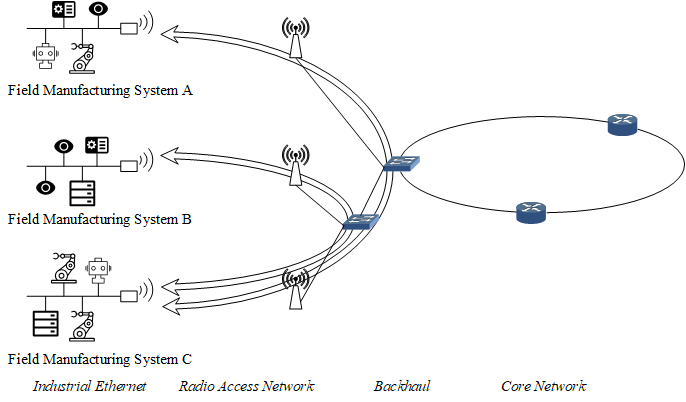
\includegraphics[width=3in]{fig11.png}
	\caption{Multi-field Manufacturing Systems Scenarios}
	% \label{fig_sim}
\end{figure}
The structure of this paper is as follows: In the first chapter, we introduce the existing synchronization algorithm and fusion architecture; In the second chapter, we analyze the clock model and error model; In chapter 3, we improved the synchronization architecture according to the model. In chapter 4, we compensated and improved the cumulative error. In chapter 5, we demonstrated the algorithm effect through simulation.
\begin{table}[htbp]
	\caption{Current Main Ethernet Protocols}
	\begin{center}
		\begin{tabular}{|c|c|c|}
			\hline
			\textbf{Protocol}& \textbf{Organization}& \textbf{Manufacturer} \\
			\hline
			EtherNet/IP
			& ODVA
			& Rockwell \\
			\hline
			PROFINET
			& PROFIBUS
			& Siemens \\
			\hline
			EtherCAT
			& EtherCAT Association
			& Bev \\
			\hline
			POWERLINK
			& EPSG
			& ABB \\
			\hline
			CC-LINK
			& CC-Link Association
			& Mitsubishi \\
			\hline 						
		\end{tabular}
		\label{tab1}
	\end{center}
\end{table}

\begin{table}[htbp]
	\caption{Current Main Wireless Protocols}
	\begin{center}
		\begin{tabular}{|c|c|c|}
			\hline
			\textbf{Protocol}& \textbf{Delay}& \textbf{Transmission Distance} \\
			\hline
			LTE
			& 6ms
			& 400-1000m \\
			\hline
			WIFI
			& 6ms
			& 100-200m \\
			\hline
			Zigbee
			& 1-3ms
			& 10-100m \\
			\hline		
		\end{tabular}
		\label{tab1}
	\end{center}
\end{table}

\section{Synchronization Overview}
Time synchronization in TSN is based on the clock synchronization of the generalized precision time protocol (gPTP) bridge architecture of IEEE 802.1AS standard
\section{Model}

\subsection{Clock Model}
	Due to the complexity of the industrial site, the crystal oscillator of the device clock will be greatly affected, and the initial clock state and rate of change of the clock will deviate, causing errors between clocks.Specifically, the clock of one node can be expressed by
\begin{equation}
	C_i(t) = \alpha _i(t)t + \beta _i 
\end{equation}
Where $\alpha_i$ and $\beta$ are the  time-varying clock skew and constant clock offset to the reference clock. Ideally, $\alpha$=1 and $\beta$=0. The change of the slope comes from the drift of the internal crystal oscillator of the clock, and the difference in the initial state comes from the error during network initialization. The crystal frequency of the clock is affected by the specific industrial environment, such as temperature, voltage, aging degree, etc. Specifically, in the 5G-TSN bridge structure (as shown in Figure 2), 5G and TSN networks will operate in different time domains. Therefore, for the current bridge structure combined with 5G and TSN, the clock model of TSN time domain can be expressed as:
\begin{equation}
	C_i(t) = \alpha_{TSN}t + \beta _{TSN}t
\end{equation}
 Correspondingly, the clock model of 5G part can be expressed as:
 \begin{equation}
 	C_i(t) = \alpha_{5G}t + \beta _{5G}t
 \end{equation}
\begin{figure}[htbp]
	\centering
	\setcounter{figure}{1}
	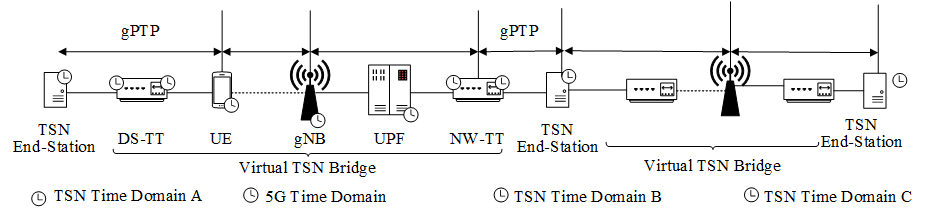
\includegraphics[width=3.5in]{fig12.png}
	\caption{5G-TSN Bridge}
	% \label{fig_sim}
\end{figure}
\subsection{Delay Model}
In the synchronization process, in addition to the accuracy of the clock, the delay between nodes is also an important factor affecting the synchronization accuracy.In the network bridge structure, the 5G network bridge is composed of all 5G wireless nodes that are relayed. Therefore, the transmission delay between the internal nodes of 5G determines the transmission delay of the network bridge, thus affecting the clock synchronization accuracy of the TSN devices at both ends.Usually,The delay can be expressed by
\begin{equation}
	Delay=D_d+D_r
\end{equation}
Where $D_d$ is the deterministic delay, which is mostly composed of transmission delay and can be eliminated by measurement, $D_r$ is the random delay, which is mostly composed of propagation delay jitter and cumulative error. According to the reference[], propagation delay jitter can be measured periodically to reduce its effect on synchronization accuracy, however, accumulated errors may have a large impact on synchronization accuracy in large-scale networks. In order to analyze the specific effects of accumulated error, it is necessary to model the queuing delay.
The internal synchronization mode of 5G network is shown in Figure 3. 5G wireless nodes synchronize by receiving Sync messages from the base station. When multiple nodes synchronize with the same base station at the same time, queuing delay will occur. To calculate the expected value of the queuing delay, firstly, the queue generated by the non-clock-synchronous traffic arriving in batches at the switch is calculated, and the expected value of the series is obtained by calculating the generating function of the series. Then, the queue delay of the clock-synchronous flow in the case of background traffic is analyzed. To get the expected length of the queue. The calculation of background traffic adopts the non-preemptive consideration, which is more in line with the actual situation. The non-clock synchronous traffic queue and clock synchronous traffic queue are modeled, and the queuing theory is used to model and solve the Markov chain. The maximum queue value is m, the packet arrival rate is $\lambda $, the packet processing rate is $\mu $, and a is the distribution of the number of packets arriving. The steady-state equation listed according to the Markov chain is:
\begin{equation}
	p_i\left( \lambda +i\cdot \mu \right) =\sum_{j=0}^i{p_j\cdot \lambda \cdot a_{i-j}+p_{i+1}\left( i+1 \right) \cdot \mu\,\, 0\leqslant i<m}
\end{equation}
\begin{equation}
		p_i\left( \lambda +m\cdot \mu \right) =\sum_{j=0}^i{p_j\cdot \lambda \cdot a_{i-j}+p_{i+1}m\cdot \mu}\,\, m\leqslant i
\end{equation}
Where $c=\mu/\lambda $.We assume that when $k$ packets arrives at the base station,there are $v$ non-clock synchronous packets in the systemthere,so there can be 3 cases:

Case 1:  $v<m$,$k<m-v$. $QueueLength = 0$

Case 2: $v<m$,$k>m-v$. $QueueLength = k+v-m$

Case 3: $v>m$. $QueueLength = k$

Based on these three cases, the expected value of queuing delay can be obtained by solving the Markov chain and summing with the full probability formula:
\begin{equation}
	L_q=P_0\cdot \sum_{i=0}^m{\left( k-m+i \right) \cdot \frac{\left( \lambda /\mu \right) ^i}{i!}+P_0\cdot \frac{k-m}{m!}\cdot \frac{\rho ^m}{v!\left( 1-\rho ^m \right)}}
\end{equation}
Where $\rho=1/c$. According to the 5G protocol standard 3GPP TS 22.104 for large-scale application scenarios[], when the service area $\in (10,20)km^2$, the upper limit of synchronization nodes in a single time domain is 100, and the queuing delay expectation can be less than 250ns after it is brought into the model. Since the synchronization accuracy is required to be $1\mu s$, we make reasonable assumptions in this case: The random queuing delay part has negligible influence on the synchronization accuracy, and only the fixed delay part has influence on the synchronization accuracy.
\section{Synchronization Architecture}
\subsection{Network Structure}
After the model derivation in the last chapter, we designed the overall synchronization architecture of heterogeneous network on this basis. Given the clock model's different time-domain models, the industrial Ethernet network is divided into different wired islands, in which the 5G network acts as the bridge. For time synchronization in integrated 5G and TSN systems, two main clock models are considered in 3GPP. These clock models comply with the IEEE 802.1AS standard and are described below. Boundary Clock -- In the Boundary clock solution, the 5G Radio Access Network (RAN) has direct access to the TSN master clock. The 5G RAN provides timing information to the user equipment (UE) through its own signaling and procedures. UE synchronizes TSN devices based on periodic information. Transparent clock - In a transparent clock solution, time synchronization is achieved by exchanging PTP messages. Any intermediate 5G or TSN entity between the TSN main console and the TSN device will update the PTP message to update the time being spent in the entity.

So 5G networks serve as transparent clocks and wired networks as boundary nodes. 5G RAN has direct access to TSN Master Time. This can be done through a direct connection to the TSN master clock or through an underlying transport network that supports PTP. This can reduce the transmission overhead of TSN timestamps in 5G networks. 

At the same time, in order to meet the requirements of assumptions (and also to meet the requirements of communication protocols), the number of wireless nodes in each network bridge should not be more than 100. When the number of nodes is more than this number, a new boundary node will be established to split the network bridge.

The overall architecture diagram is shown in Figure 3:
\begin{figure}[htbp]
	\centering
	\setcounter{figure}{2}
	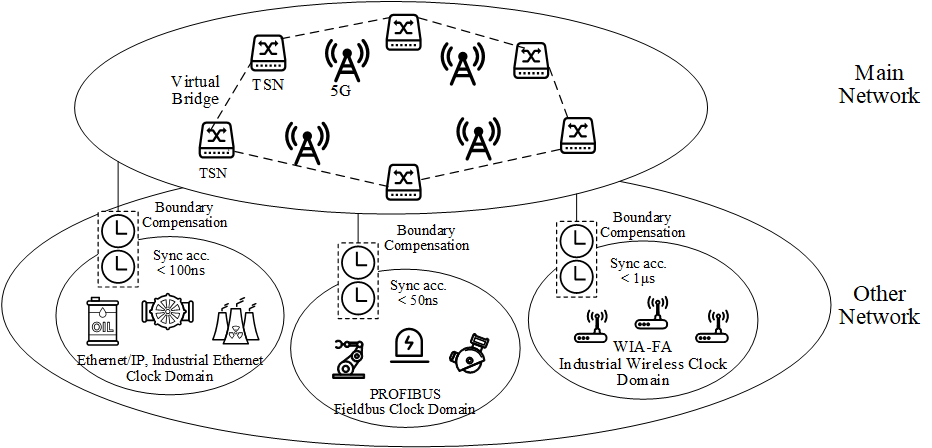
\includegraphics[width=3.5in]{fig17.png}
	\caption{Schematic of slot allocation in the TAS model}
	% \label{fig_sim}
\end{figure}
\subsection{Synchronization Mechanism}
The initial synchronization of the wired part adopts GPTP synchronization scheme, the initial synchronization of the wireless part is completed through broadcast synchronization. The root node imparts the count $k=0$ into the broadcast of the synchronization message, and the receiving node sets the count $k+1$ to the local level and sends the broadcast synchronization message containing $k+1$ to the next level. Each interval is one time slot. The slave clock receives the reference timestamp $G$ from the master clock through several intermediate ones and records the local time $L$. The estimation of frequency difference and clock deviation is obtained by linear regression after the exchange of several sets of timestamps. The intermediate forwarding node will be treated as a transparent clock. Finally, the correction time of each wireless node can be expressed as:
\begin{equation}
	\widehat{L}=L\left(1+\frac{\widehat{\sigma}}{f_0}\right)-\widehat{o}+\left[\frac{G_0-L_0}{T_{\text {slot }}}\right] T_{\text {slot }}
\end{equation}
Where $\widehat{\sigma}$ is the estimation of frequency difference and $\widehat{o}$ is the estimation of clock deviation.After initial synchronization, the overall clock model can be preliminarily equivalent to the model in Chapter 3:

$C_i(t) = \alpha_{TSN}t + \beta _{TSN}t$ 

$C_i(t) = \alpha_{5G}t + \beta _{5G}t$
\section{Synchronization Error}

\subsection{Frequency Domain Synchronization Error}

According to the definition of synchronization accuracy in 5G, synchronization accuracy $\sigma$ denotes the standard deviation of clock synchronization error, which can be expressed as phase error $\epsilon$. Therefore, we can define the synchronization accuracy in terms of the standard deviation of the phase error, i.e.

$$\sigma = \sqrt{\frac{1}{N}\sum_{i=1}^N(\epsilon_i - \bar{\epsilon})^2}$$

where $N$ denotes the number of samples, $\epsilon_i$ denotes the phase error at the $i$th sampling moment, and $\bar{\epsilon}$ denotes the average of the phase errors at all sampling moments.

Now we need to establish a mathematical relationship between the synchronization accuracy and the carrier interval. According to the previous derivation, the phase error can be expressed as $\epsilon = 2\pi\Delta t / T_c$, where $\Delta t$ denotes the clock synchronization error and $T_c$ denotes the carrier period. Therefore, we can express the standard deviation of the phase error $\sigma$ as

$$\sigma = \sqrt{\frac{1}{N}\sum_{i=1}^N\left(\frac{2\pi\Delta t_i}{T_c} - \bar{\epsilon}\right)^2}$$

Deforming the above equation yields.

$$\sigma = \frac{\pi}{\sqrt{2}T_c}\cdot\sqrt{\frac{1}{N}\sum_{i=1}^N\left(\frac{T_c}{\Delta}\cdot\Delta t_i - \bar{\epsilon}\right)^2}$$ 

According to the above equation, we can see that there is an inverse relationship between the synchronization accuracy and the carrier interval, i.e., the synchronization accuracy decreases with the increase of the carrier interval.

Carrier bandwidth affects the synchronization accuracy of 5G and time-sensitive TSN networks, from a frequency domain perspective. Specifically, the wider the carrier bandwidth, the higher the frequency resolution and therefore the more accurate the measurement of clock synchronization differences, thus improving synchronization accuracy. In the frequency domain, the impact on clock synchronization accuracy can be described in terms of power spectral density, and the carrier bandwidth is a key parameter affecting the power spectral density. Therefore, in 5G and TSN networks, the choice of carrier bandwidth is very important and can affect the clock synchronization accuracy and the performance of the whole network.

In clock synchronization, the local clock frequencies of the sender and receiver may be slightly different, so a time offset $\Delta t$ will occur. If this time offset is small, it can be considered as a small angle, and then using the approximation formula $$\sin(x) \approx x$$ for the sine function (where$x$ is expressed in radians and $x$ is small), we get

$$\sin(\Delta\theta) \approx \Delta\theta \approx \frac{\Delta t}{T_s}$$

where $\Delta\theta$ is the phase deviation of clock synchronization and $T_s$ is the clock synchronization period.

Since the synchronization accuracy is half of $\Delta t$, we can obtain
$$T_s = \frac{\Delta T}{2} = \frac{1}{2}\left(\frac{|\Delta t_{tx} - \Delta t_{rx}|}{2}\right)$$
where $\Delta T = |\Delta t_{tx} - \Delta t_{rx}|$ is the clock synchronization error, and $t_{tx}$ and $t_{rx}$ are the transmit and receive timestamps, respectively.
Therefore, the approximation formula for the sine function is one of the reasons why the synchronization accuracy can be expressed as the above formula.

In 5G networks with time-sensitive networks (TSN), there is a certain mathematical relationship between clock synchronization accuracy and carrier interval. Assuming that $T_s$is the time synchronization error (i.e., clock synchronization accuracy) and $T_c$ is the carrier interval, the relationship between them can be expressed as follows
\begin{equation}
	T_s = \frac{1}{2\pi f_c}\cdot arctan\left(\frac{2\pi f_c}{\Delta}\right)
\end{equation}

where $f_c$ denotes the carrier frequency and $\Delta$ denotes the transmission delay of the synchronization message.

The derivation of the formula is as follows.
According to the nature of the sine function, the synchronization accuracy $T_s$ can be expressed as
\begin{equation}
	T_s = \frac{\Delta T}{2} = \frac{1}{2}\left(\frac{|\Delta t_{tx} - \Delta t_{rx}|}{2}\right)
\end{equation}
where $\Delta t_{tx}$ denotes the timestamp of the synchronization message sent by clock A and $\Delta t_{rx}$ denotes the timestamp of the synchronization message received by clock B.
Consider the transmission delay $$\Delta$$ of the synchronization message, which consists of the following components.
\begin{equation}
	\Delta = \Delta_{tx} + \Delta_{prop} + \Delta_{rx}
\end{equation}
where $\Delta_{tx}$ is the transmission delay of the synchronization message from clock A to the switch, $\Delta_{prop}$ is the propagation delay of the synchronization message from the switch to clock B.
$\Delta_{rx}$ is the delay time delay of the synchronization telegram received from the B clock.
For the transmission delay $\Delta$ of a synchronous telegram, it can be expressed in terms of the carrier interval $T_c$ as:
\begin{equation}
	\Delta = k \cdot T_c 
\end{equation}

where $k$ is a constant indicating the transmission time of synchronous messages as a percentage of the carrier interval.
Combining the above two equations, we get:
\begin{equation}
	T_s = \frac{1}{2}\left(\frac{|k \cdot T_c + \Delta t_{tx} - \Delta t_{rx}|}{2}\right)
\end{equation}
By the definition of $T_c$, we have $T_c = \frac{1}{f_c}$, that is: $f_c = \frac{1}{T_c}$
Substituting $f_c$ into the above equation, we get.
$$T_s = \frac{1}{2\pi f_c}\cdot arctan\left(\frac{2\pi f_c}{\Delta}\right)$$
where $f_c$ denotes the carrier frequency and $\Delta$ denotes the transmission delay of the synchronization message.Thus, the relationship between the carrier interval $T_c$ and the clock synchronization accuracy $T_s$ can be expressed as the above equation. 

This equation shows that the smaller the carrier spacing, the higher the clock synchronization accuracy, but there is a limit to the accuracy improvement, and $T_s$ converges to a fixed value when $\Delta$ tends to 0.
This equation illustrates the effect of carrier spacing on clock synchronization accuracy in 5G networks with TSNs. Specifically, when the carrier frequency $f_c$ is fixed, increasing the carrier interval $T_c$ decreases the clock synchronization accuracy $T_s$, while decreasing the carrier interval $T_c$ increases the clock synchronization accuracy.


In the process of single-hop transmission, formula 6 shows that the factor affecting transmission delay is time slot length, and the impact caused by cumulative errors depends on the size of time slots in the synchronization process, which determines the upper limit of the accuracy of synchronization accuracy. In 5G networks, the size of time slots can be optimized by carrier allocation.
As shown in Figure 5, the length of wireless frame and subframe in 5G is the same. Wireless frame is 10ms, and the length of subframe is 1ms. The number of ofdm symbols contained in a time slot in 5G is 14. SSBS (clock synchronization messages) fixed occupy 4 ofdm symbols, so the duration and period of SSBS are different under different subcarrier intervals, and the interval of 5G subcarriers can be adjusted. By taking advantage of the distributable property of the subcarrier interval in 5G network, the number of subcarriers and the symbol length of ofdm can be reduced by increasing the subcarrier interval, so as to reduce the delay and cumulative error. Under a certain general transmission environment, the coherence bandwidth is the same. 

However, increasing the carrier spacing can also cause the following problems:
\begin{itemize}
	\item Reduced spectral efficiency: The larger the carrier interval, the smaller the amount of data that can be transmitted on each carrier, and the lower the spectral efficiency.
	
	\item Reduced anti-interference capability: The larger the carrier spacing, the larger the channel width, and the larger the BER when encountering interference sources.
	
	\item Increased power consumption: If the BER is to be guaranteed low, the signal power needs to be enhanced, which will lead to increased power consumption.
	
	\item Waste of resources: A large carrier spacing may cause some spectrum resources to be wasted.
\end{itemize}
Therefore, choosing a suitable carrier spacing and using an equalizer to compensate is the key to achieve high precision 5G+TSN synchronization.


\begin{figure}[htbp]
	\centering
	\setcounter{figure}{2}
	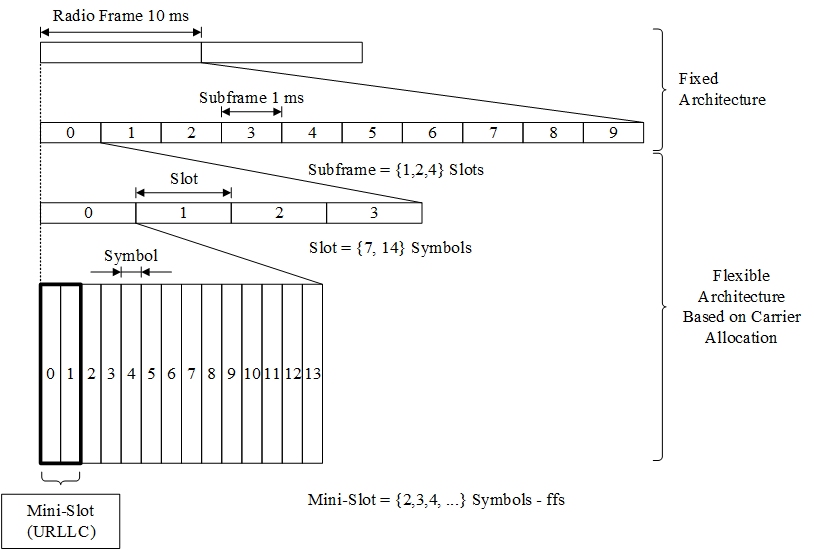
\includegraphics[width=3in]{fig14.png}
	\caption{5G carrier structure}
	% \label{fig_sim}
\end{figure}
\subsection{Multihop Error}
When multiple Bridges are connected to each other in the network, as shown in Figure 1, the cumulative error will be further amplified and the time stamp needs to be compensated and corrected. In calculation, multiple network Bridges can be abstracted as one for processing, and TSN time domain at both ends can be abstracted as master-slave nodes.
As shown in Figure 5, during network estimation, the local time of wired and wireless sides can be expressed as:
\begin{eqnarray}
	\begin{aligned}
		&t_{(\text {wired})}=\left(\alpha_{1}+\sigma_{1}\right) t+\beta_{1}+\delta_{1}\\
		&t_{(\text {wireless })}=\left(\alpha_{2}+\sigma_{2}\right) t+\beta_{2}+\delta_{2}\\
	\end{aligned}
\end{eqnarray}
Where $\alpha_1,\sigma_{1}$is the frequency synchronization correction estimate and error on the wired side, $\alpha_2,\sigma_{2}$is the frequency synchronization correction estimate and error on the wireless side, $\beta_1,\delta_{1}$is the time bias synchronization correction estimate and error on the wired side, $\beta_2,\delta_{2}$is the estimated value and error of the time-bias synchronization correction on the wireless side, and t is the time of the reference clock. Due to the accuracy difference of time bias and frequency estimation on both sides, the boundary synchronization error will be caused when the clock synchronization of wire and wireless timestamp exchange is carried out.

For the left wired master clock, the sync message sent contains a timestamp of time $t_1$, At this point the corresponding reference time should be $t_1^{ref}$, when this message arrived wireless side from the clock, the node will receive and record the timestamp $t_2$, the timestamp values can be expressed as: 
\begin{equation}
	t_{2}=(t_1^{ref}+delay)(\alpha_{2}+\sigma_{2})+\beta_{2}+\delta_{2}
\end{equation}
\begin{equation}
	t_1^{ref}=\frac{t_{1}-\beta_{1}-\delta_{1}}{\alpha_{1}+\sigma_{1}}
\end{equation}

Similarly, on the wireless network side, the wireless network node records the timestamp $t_3$ after receiving the $Sync$ message and sends the message $Delay\_Req$. Then the wired network node records the timestamp $t_4$ after receiving $Delay\_Req$. the value of the timestamp can be expressed as:
\begin{equation}
	t_{4}=(t_3^{ref}+delay)(\alpha_{1}+\sigma_{1})+\beta_{1}+\delta_{1}
\end{equation}
\begin{equation}
	t_3^{ref}=\frac{t_{3}-\beta_{2}-\delta_{2}}{\alpha_{2}+\sigma_{2}}
\end{equation}

Thus the transmission delay between the two network nodes can be expressed as:

	\begin{equation}
		\begin{gathered}
			2  delay =t_{2}-t_{1}+t_{4}-t_{3} \\
			=m\left(t_{2}-t_{1}+t_{4}-t_{3}\right)-(m-1 / m)\left(\beta_{1}+\delta_{1}\right)+(m-1 / m)\left(\beta_{2}+\delta_{2}\right) \\
			 \approx m\left(t_{2}-t_{1}+t_{4}-t_{3}\right)-(m-1 / m)\left(\beta_{2}+\delta_{2}\right)\\
		\end{gathered}
	\end{equation}

\begin{equation}
		m=\frac{\alpha_{2}+\sigma_{2}}{\alpha_{1}+\sigma_{1}}		
\end{equation}
In Equation 14, since the synchronization error of the wired part is much smaller than that of the wireless part, it is neglected.
Note that the calculation of the timestamp and clock parameters should be done on the side of the wired network, i.e., the TSN node, and then the result is sent to the 5G network node via the $Delay\_Resp$ message. The synchronization algorithm involves floating-point division, and since TSN network nodes have higher accuracy in floating-point calculation, all of them are done in the head (TSN) part, which can effectively improve the synchronization accuracy and reduce the computational complexity of 5G nodes.

\begin{figure}[htbp]
	\centering
	\setcounter{figure}{3}
	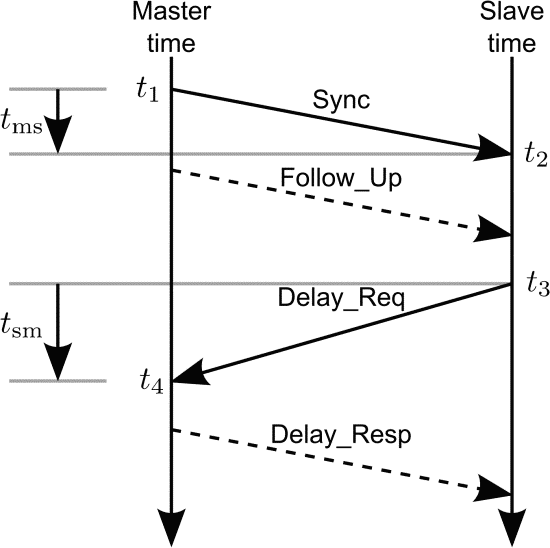
\includegraphics[width=3in]{fig10.png}
	\caption{Synchronization process}
	% \label{fig_sim}
\end{figure}
\section{Simulation Results}
Based onn the literature [3], it is proposed that in the intelligent factory integrated with the industrial network and 5G network in the future, there are multiple industrial Ethernet application scenarios that work cooperatively through the 5G network in the time domain. So we proposed a general simulation scenario, shown in Fig. 5, models the cooperative interaction of several mobile robots. A typical use case for future factories, that requires precise time synchronization of sevaral wired networks across wireless links.
\begin{figure}[htbp]
	\centering
	\setcounter{figure}{4}
	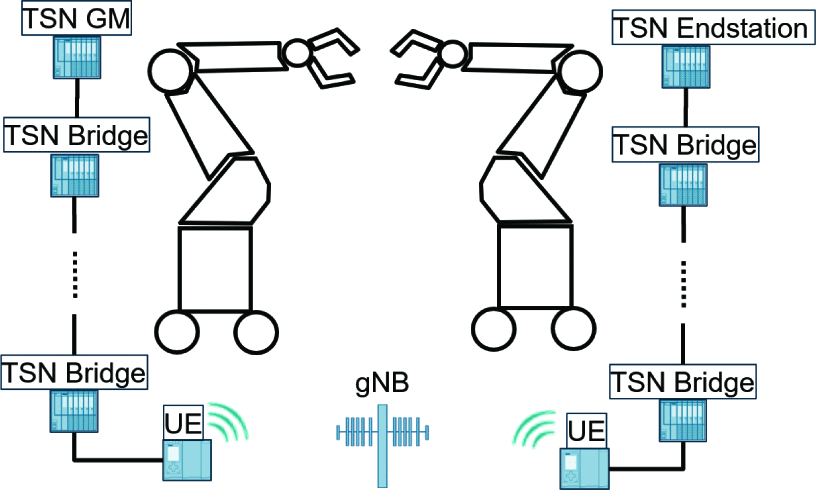
\includegraphics[width=3in]{fig5.png}
	\caption{Synchronization process}
	% \label{fig_sim}
\end{figure}

\subsection{Single-hop Simulation}

Single-hop synchronization is implemented in matlab for baseband simulation, not involving RF content, the receiver input signal rxWaveform has been IQ road data, SSB can only be in the synchronization grid, synchronization grid is used to configure the basic frequency location of the synchronization / broadcast signal, is an absolute frequency. rxWaveform can also be understood as the receiver has been from the synchronization grid this frequency The baseband data obtained after down-converting to baseband and completing A/D sampling, the baseband data is determined by a series of algorithms to determine if there is an SSB synchronization block inside this data. If there is, it means that there is a synchronization block in this synchronization grid, and it has been found, and the MIB is recovered. The synchronization method is set to "time-frequency two-dimensional search" according to the 5G protocol, and the coarse frequency bias estimation and determination of NID2 is done by traversing the three cases of NID2. matlab5G toolbox is set to 1/2*scs for the search step, because the range that can be estimated by the CP-based CFO estimation technique is the subcarrier interval multiplied by [-0.5,0.5), and this technique cannot be used to estimate integer multiplicative frequency bias. So the frequency spacing error needs to be estimated to within the subcarrier spacing times [-0.5,0.5) before the CP-based CFO estimation technique can be used.
Then, after that, we will not use 1/2*scs but choose 15khz to compare the accuracy of the frequency difference estimation.
For channel equalization at low carrier spacing, MMSE equalization, which is a ZF equalizer that takes into account the noise, will be used here, assuming that the transmitter sends a guide sequence x = [1,1,1,1,1,1], [1,1,1,1,1] arrives at the receiver after passing through the channel, which is assumed to be called y. The receiver compensates by the y already received, and the H already obtained by channel estimation before this, to the effect of the channel on the signal, thus recovering x more efficiently.

The simulation experimental results are shown in Fig. 5 and Fig. 6. The synchronization errors at different carrier intervals are shown in Fig. 5, and the BER at low carrier intervals after equalizer compensation is shown in Fig. 6.As shown in the figure, the synchronization accuracy is significantly improved with low carrier spacing and with equalizer compensation.
\begin{figure}[htbp]
	\centering
	\setcounter{figure}{6}
	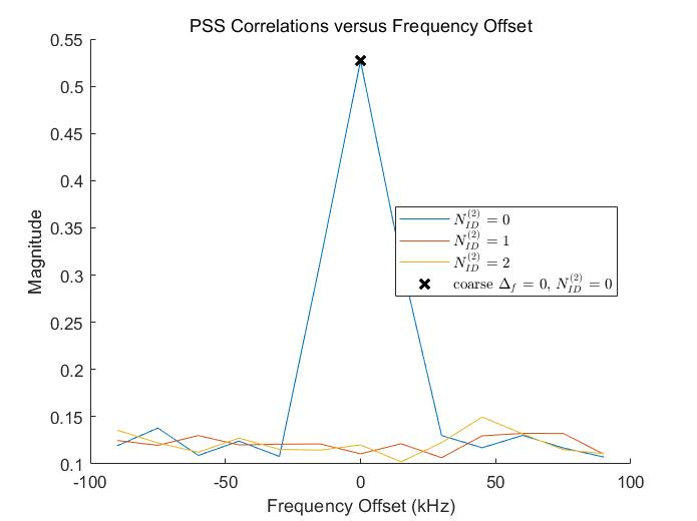
\includegraphics[width=3in]{fig6.png}
	\caption{frequency offset at different carrier intervals}
	% \label{fig_sim}
\end{figure}
\begin{figure}[htbp]
	\centering
	\setcounter{figure}{8}
	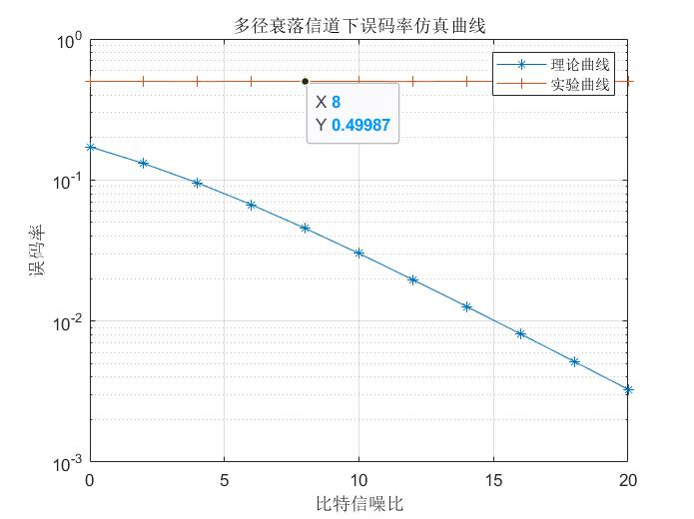
\includegraphics[width=3in]{fig8.png}
	\caption{BER before equalizer compensation}
	% \label{fig_sim}
\end{figure}
\begin{figure}[htbp]
	\centering
	\setcounter{figure}{9}
	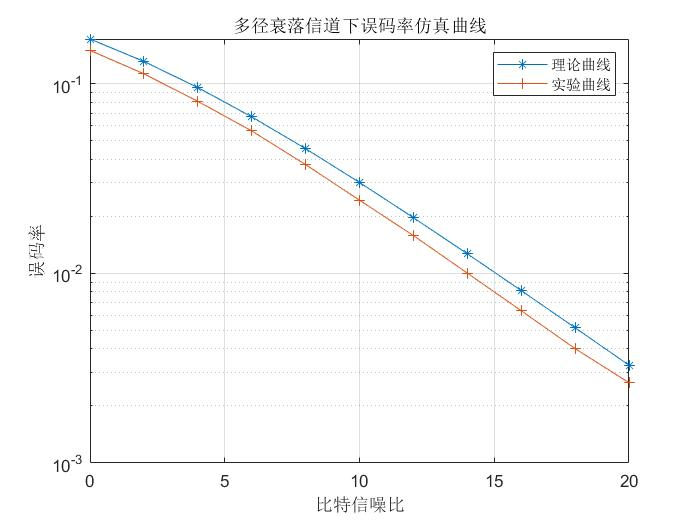
\includegraphics[width=3in]{fig9.png}
	\caption{BER after equalizer compensation}
	% \label{fig_sim}
\end{figure}
\subsection{Multihop Simulation}
We model each mobile robot as a TSN endstation, connected to a 5G UE via a variable number of TSN Bridges (here: transparent clocks). Every device, both TSN and 5G, is based on the omnet Node class. For every node, a clock instance according to section III clock modle. The rest of the setup differs between TSN and 5G devices:
The TSN nodes are connected using the Carrier Sense Multiple Access (CSMA) channel model. ns-3 does not provide a real ethernet model, however the CSMA channel model supports layer 2 communication and is a sufficiently close approximation of ethernet for our purpose.
\begin{itemize}
	\item The gPTP procedures are defined in a separate class and installed on each node. We differentiate between ordinary and transparent clocks. This determines how a node interacts with the different gPTP messages. Every TSN node will initiate the peer delay messaging process to its neighbors. Only the ordinary clock acting as the master clock will initiate the synchronization messaging process.
	\item The 5G devices have to act as a gateway between the TSN and 5G networks. To achieve that, they are made up of two nodes. One node is connected to the CSMA channel and acts as the wired (ethernet) port. The other node acts as the 5G module and is connected to the wireless channel. Both nodes share the same local clock instance and essentially act as one device. The TSN translator functionalities are also defined in a separate class and installed on these 5G nodes.
	
	The 5G internal communication uses the 5G LENA module [16]. This module focuses on the PHY and MAC layers, based on the 3GPP Rel. 15 non-standalone version of 5G. Higher layers reuse the existing LENA lte module.
	
	The 5G LENA module provides a wireless channel implementation and supports different frame structures and frequency bands. For the 5G-internal traffic, UDP/IP communication is used. The specific configuration setup used for our 5G LENA implementation is given in Table
\end{itemize}


\bibliography{cx.bib}
\bibliographystyle{IEEEtran}
\end{document}
